\section{Modelado Matemático 2}\index{Modelado!Modelado Matemático 2}
En el modelo matemático se encuentran incluidos todos los factores que intervienen en el comportamiento del robot y dependiendo del tipo de modelado, se puede obtener una simulación del comportamiento real del robot.\\

La cinemática estudia el movimiento de algún sistema sin tomar en cuenta las fuerzas externas que producen este movimiento o que pudieran afectarlo. En el caso del estudio cinemático del robot, se describe su movimiento de manera analítica mediante una función que relaciona la posición y orientación del punto final del robot con los valores de cada una de las articulaciones del robot. Existen dos tipos de estudios cinemáticos: Cinemática Directa y Cinemática Inversa.\\

El problema cinemático\index{cinemática} directo se refiere a expresar la posición y orientación del punto final del robot a partir de los valores conocidos de las articulaciones.\\

El problema cinemático inverso consiste en conocer los valores que se le deben asignar a cada una de las articulaciones para llegar a la posición y orientación deseada.\\

La cinemática del robot se representa con la llamada Matriz de Transformación Homogénea. Esta matriz representa la posición y la orientación relativa entre dos eslabones seguidos o unidos. Para trabajar con esta matriz es necesario establecer un sistema de coordenadas. Una herramienta muy utilizada para la descripción cinemática de robots es el algoritmo de Denavit-Hartenberg (D-H). Con la utilización de esta herramienta se modela cinemáticamente el robot. El robot tiene un total de 10 grados de libertad divididos en 5 para cada pierna, sin embargo, las piernas son iguales físicamente y su movimiento es similar, así que en realidad sólo es necesario modelar una pierna de 5 grados de libertad. \\

Los parámetros a utilizar en el algortimo de D-H se muestran a continuación.\\

\newpage

\begin{figure}[h]
	\centering
		\fbox{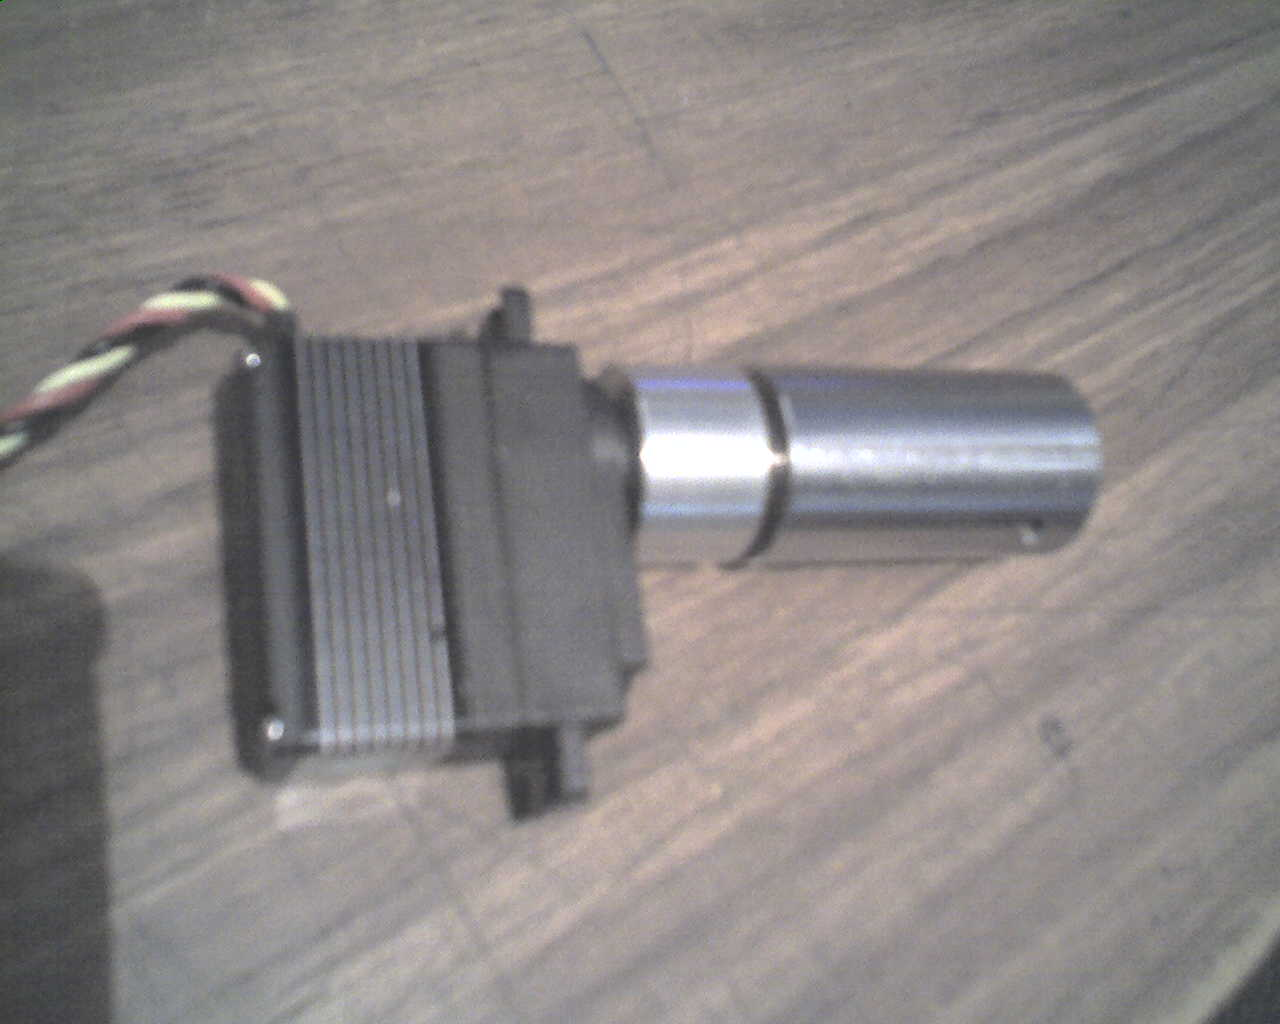
\includegraphics[scale=0.25]{imagenes/img106.jpg}}
		\caption{Ejes coordenados.}\label{fig:DH}
\end{figure}

\begin{table}[h]
	\centering
		\begin{tabular}{|c|c|c|c|c|}
		\hline
			$Eslabon_{i}$	&	$a_{i}$	&	$d_{i}$	&	$\alpha_{i}$ & $\theta_{i}$	\\
			\hline
			0	&	0	&	0	&	0	&	0	\\
			\hline
			1&a1&0&90&q1\\
			\hline
			2&a2&0&0&q2\\
			\hline
			3&a2&0&0&q3\\
			\hline
			4&a1&0&90&q4\\
			\hline
			5&0&0&0&q5\\
			\hline
		\end{tabular}
	\caption{Parámetros de D-H.}
	\label{tab:DH}
\end{table}

Las matrices de transformación Homogéneas obtenidas para cada uno de los eslabones son:\\

\begin{center}

$T_0^1 $= 	\begin{math}
				\left[
				\begin{array}{cccc}
			   	cos(q_1)&               0&         sin(q_1)& 62.82cos(q_1)\\
         sin(q_1)&               0&         cos(q_1)& 62.82sin(q_1)\\
               0&               1&               0&            0 \\
               0&               0&               0&            1

				\end{array}
				\right]
				\end{math}\\
				
\vspace{1cm}

$T_1^2 $= 	\begin{math}
				\left[
				\begin{array}{cccc}
			   	cos(q_2)&	  		 -sin(q_2)&								0&			68.29cos(q_2)\\
          sin(q_2)&          \cos(q_2)&                0& 		 68.29\sin(q_2)\\
                0&                0&                1&                0\\
                0&                0&                0&                1
				\end{array}
				\right]
				\end{math}\\

\vspace{1cm}				

$T_2^3 $= 	\begin{math}
				\left[
				\begin{array}{cccc}
			   	cos(q_3)&	  		 -sin(q_3)&								0&			68.29cos(q_3)\\
          sin(q_3)&          cos(q_3)&                0& 		 68.29sin(q_3)\\
                0&                0&                1&                0\\
                0&                0&                0&                1

				\end{array}
				\right]
				\end{math}\\
				
\vspace{1cm}				

$T_3^4 $= 	\begin{math}
				\left[
				\begin{array}{cccc}
			   	cos(q_4)&               0&         sin(q_4)& 62.82cos(q_4)\\
         sin(q_4)&               0&         cos(q_4)& 62.82sin(q_4)\\
               0&               1&               0&            0 \\
               0&               0&               0&            1

				\end{array}
				\right]
				\end{math}\\			

\vspace{1cm}

$T_4^5 $= 	\begin{math}
				\left[
				\begin{array}{cccc}
			   	cos(q_5)&	  		 -sin(q_5)&								0&			0)\\
          sin(q_5)&          cos(q_5)&                0& 		 0\\
                0&                0&                1&      0\\
                0&                0&                0&      1

				\end{array}
				\right]
				\end{math}\\
				
				\newpage
				
			
			
{\footnotesize
\begin{center}
				$T_0^5 $= 	
	\begin{math}
\left[
		\begin{array}{ccc}
		\left(\begin{array}{c}
		 cos(q_1)cos(q_5)cos(q_2+q_3+q_4)\\
			   +sin(q_1)sin(q_5)
			   \end{array}\right)&\left(\begin{array}{c}
			   -cos(q_1)sin(q_5)cos(q_2+q_3+q_4)\\
			   +sin(q_1)cos(q_5)
			   \end{array}\right)&cos(q_1)sin(q_2+q_3+q_4\\
			   && \\
\left(\begin{array}{c}
sin(q_1)cos(q_5)cos(q_2+q_3+q_4)\\
-sin(q_1)sin(q_5) \end{array}\right)&\left(\begin{array}{c}
-sin(q_1)sin(q_5)cos(q_2+q_3+q_4)\\
-cos(q_1)cos(q_5)\end{array}\right)&-sin(q_1)sin(q_2+q_3+q_4)\\
   && \\
cos(q_5)sin(q_2+q_3+q_4)&-sin(q_5)sin(q_2+q_3+q_4)&-cos(q_2+q_3+q_4)\\
 & & \\
0&0&0
		\end{array}
				\right]
				\end{math}\\
\end{center}
}
\end{center}

Con este modelo matemático es posible generar trayectorias y así analizar la etapa de caminado. También es posible realizar un control de movimiento, sin embargo, este control no ofrecerá la mejor solución, ya que al resolver el problema cinemático, no se están considerando algunos factores que podrían afectar al modelo, es por eso que se decide realizar también un modelado dinámico del sistema.

\section{Nuevos métodos}

11.	On the last page of the Delegation of Control Wizard, click Finish to exit the wizard.
Delegating Create all Child Objects and Delete all Child Objects control of the OU to the application pool identity account for Central Administration enables administrators to enable email for a list. After these controls have been delegated, administrators cannot disable email for the list or document library because the Central Administration account tries to delete the contact from the whole OU instead of from the list.
To avoid this problem, you must add Delete Subtree permissions for the application pool identity account for Central Administration. Use the following procedure to add these permissions. After this procedure is complete, you can disable incoming email for a list.
To add Delete Subtree permissions for the application pool identity account for Central Administration

1.	Verify that the user account that is performing this procedure is a member of the Domain Administrators group or the Enterprise Administrators group in AD DS, or a delegated authority for domain administration.
2.	In Active Directory Users and Computers, click the View  menu, and then click Advanced Features.
3.	Right-click the OU, and then click Properties.
4.	In the Properties dialog box, click the Security tab, and then click Advanced.
5.	In the Permission Entries area, double-click the application pool identity account for Central Administration.
If the application pool identity account is listed more than once, select the first one.
6.	In the Permissions area, select Allow, for Delete Subtree.
7.	Click OK to close the Permissions dialog box.
8.	Click OK to close the Properties dialog box.
9.	Click OK to close Active Directory Users and Computers.
After you add these permissions, you must restart Internet Information Services (IIS) for the farm.
For more information, see Active Directory Users, Computers, and Groups in the TechNet Library.

Configure DNS Manager\nomenclature{DNS}{ servicod e de nominioo de nombres}

If you are using Exchange Server and are routing email internally in your organization, you must create a host (A) resource record in DNS Manager to associate DNS domain names of computers (or hosts) to their IP addresses. Your organization might already have a configured DNS Manager and an A resource record. If not, then use the following procedure.
To create an A resource record for a subdomain

1.	Verify that the user account that is performing this procedure is a member of the Administrators group on the local computer.
2.	In DNS Manager, select the forward lookup zone for the domain that contains the subdomain for SharePoint 2013.
3.	Right-click the zone, and then click New Host (A or AAAA).
4.	In the New Host dialog box, in the Name text box, type the host or subdomain name for SharePoint 2013.
5.	In the Fully qualified domain name (FQDN) text box, type the FQDN for the server that is running SharePoint 2013. This is typically in the format subdomain.domain.com.
6.	Ensure that the domains that are listed under the SMTP server in IIS match the FQDN of the server that receives email. If they do not match, you must create a local domain. For instructions, see To create a local domain later in this article.

7.	In the IP address text box, type the IP address to which you want the FQDN to resolve.
8.	Click Add Host.
9.	In the message that confirms the creation of the host record, click OK.
10.	In the New Host dialog box, click Done.
The A resource record now appears in DNS Manager.
If you use the E-mail server display address option and if the email address to which you are sending email messages is not the same as your server name, you must create a local domain.
To create a local domain
1.	Click Start, point to Administrative Tools, and then click Internet Information Services (IIS) 6.0 Manager.
2.	In IIS Manager, expand the SMTP server.
3.	Right-click Domains, and on the Action menu, point to New, and then click Domain.
4.	In the New SMTP Domain Wizard dialog box, select Alias, and then click Next.

5.	In the Domain Name area, in the Name box, type the address of the mail that is to be received by this domain.
This address must be the same as the one that you specified in step 4 in To create an A resource record for a subdomain, and in step 6b in To configure incoming email in an advanced scenario.
6.	Click Finish.
7.	In the message that confirms the creation of the host record, click OK.
8.	Restart the SMTP server so that all email messages that are still in the Queue folder move to the Drop folder. The messages are then sent by the Windows SharePoint Services Timer service to their destination list or library.

 	Note:
If you are routing email from outside your organization to an SMTP server, you must use an MX record. For more information, see Add a mail exchanger (MX) resource record to a zone in the
